\documentclass[aspectratio=169,10pt]{beamer}
\usetheme{moloch}
\molochset{progressbar=frametitle, titleformat=regular}
\setbeamertemplate{page number in head/foot}[totalframenumber]
\molochset{block=fill}

\usepackage[T1]{fontenc}
\usepackage[utf8]{inputenc}
\usepackage{lmodern}
\usepackage{amsmath,amssymb}
\usepackage{booktabs}
\usepackage{array}
\usepackage{graphicx}
\usepackage{xcolor}
\usepackage{listings}
\usepackage{fontawesome5}
\usepackage{tikz}
\usetikzlibrary{positioning,arrows.meta,calc,fit}

\definecolor{temBlue}{HTML}{356CA5}
\definecolor{temGreen}{HTML}{4F8A5B}
\definecolor{temOrange}{HTML}{D9892B}
\definecolor{temViolet}{HTML}{8064A2}
\definecolor{temGray}{HTML}{F2F4F7}
\definecolor{temDark}{HTML}{343A40}
\definecolor{temCodeString}{HTML}{2E7D50}
\definecolor{temCodeComment}{HTML}{6C757D}

\newcommand{\smallcode}[1]{\texttt{\footnotesize #1}}
\newcommand{\pct}[1]{\texttt{#1\%}}
\newcommand{\mi}{\,MiB}
\newcommand{\gibi}{\,GiB}

\lstdefinelanguage{Bazel}{
  sensitive=true,
  morekeywords={cc_binary,name,srcs,linkshared,malloc,deps},
  morestring=[b]",
  morecomment=[l]{\#}
}

\lstdefinelanguage{TemShell}{
  sensitive=true,
  morekeywords={LD_PRELOAD,export},
  morestring=[b]",
  morecomment=[l]{\#}
}

\lstdefinestyle{temCode}{
  basicstyle=\ttfamily\scriptsize,
  keywordstyle=\color{temBlue}\bfseries,
  stringstyle=\color{temCodeString},
  commentstyle=\color{temCodeComment}\itshape,
  backgroundcolor=\color{black!7},
  frame=single,
  framerule=0pt,
  framesep=0.55em,
  rulecolor=\color{black!7},
  showstringspaces=false,
  columns=fullflexible,
  keepspaces=true
}

\setbeamercolor{codeblock}{fg=temDark,bg=black!7}
\newenvironment{codeblock}[1]{%
  {\scriptsize\bfseries #1}\par\vspace{0.15em}%
  \begin{beamercolorbox}[wd=\linewidth,sep=0.55em,rounded=true]{codeblock}%
  \ttfamily\scriptsize
}{%
  \end{beamercolorbox}
}

\tikzset{
  used/.style={draw=black!45,fill=temBlue!16,rounded corners=1.5pt,
    minimum height=0.46cm,minimum width=0.62cm},
  free/.style={draw=black!35,fill=temGray,rounded corners=1.5pt,
    minimum height=0.46cm,minimum width=0.62cm},
  box/.style={draw=temBlue!70!black,fill=temBlue!8,rounded corners=3pt,
    line width=0.8pt,minimum height=0.72cm,align=center,font=\small},
  greenbox/.style={draw=temGreen!70!black,fill=temGreen!10,rounded corners=3pt,
    line width=0.8pt,minimum height=0.72cm,align=center,font=\small},
  orangebox/.style={draw=temOrange!80!black,fill=temOrange!10,rounded corners=3pt,
    line width=0.8pt,minimum height=0.72cm,align=center,font=\small},
  violetbox/.style={draw=temViolet!80!black,fill=temViolet!10,rounded corners=3pt,
    line width=0.8pt,minimum height=0.72cm,align=center,font=\small},
  arrow/.style={-{Latex[length=2.4mm,width=1.7mm]},line width=0.9pt,draw=black!65},
  faintlabel/.style={font=\scriptsize,text=black!62}
}

\title{Temeraire: Redis-Reproduktion mit \"offentlichem Code}
\subtitle{Von der hugepage-aware Idee bis zum funktionierenden Experiment}
\author{Aldo Costa}
\institute{Heinrich-Heine-Universit\"at D\"usseldorf}
\date{Juli 2026}

\begin{document}

\maketitle

\begin{frame}{Was wird hier reproduziert?}
\begin{columns}[T,totalwidth=\textwidth]
  \begin{column}{0.53\textwidth}
    \begin{block}{Temeraire}
      Hugepage-bewusster Backend-Allocator f\"ur TCMalloc\\
      Hunter et al., OSDI~2021
    \end{block}
    \vspace{0.55em}
    \begin{itemize}
      \item Ziel im Paper: weniger TLB-Druck durch bessere Platzierung
      \item Ziel hier: der \"offentliche Redis~6.0.9-Case-Study-Teil
      \item Kein Google-Fleet-Experiment, keine Produktions-Telemetrie
    \end{itemize}
  \end{column}
  \begin{column}{0.43\textwidth}
    \begin{alertblock}{Arbeitsfrage}
      Kann die Redis-Methode mit \"offentlichem Code und lokaler Hardware so
      nachgebaut werden, dass die kleine Effektgr\"o{\ss}e des Papers sichtbar wird?
    \end{alertblock}
  \end{column}
\end{columns}
\note{Start with the scope. The point is not to claim the whole OSDI paper. The talk is about the public Redis reproduction and the work needed before the numbers became interpretable.}
\end{frame}

\begin{frame}{Hugepages als Ausgangspunkt}
\begin{columns}[T,totalwidth=\textwidth]
  \begin{column}{0.50\textwidth}
    \begin{itemize}
      \item Normale Seiten: 4 KiB
      \item Hugepages: 2 MiB, also 512 normale Seiten
      \item Ein Hugepage-TLB-Eintrag deckt viel mehr Speicher ab
      \item Der Gewinn ist weniger Adress\"ubersetzung, nicht ein gr\"o{\ss}erer Cache
    \end{itemize}
  \end{column}
  \begin{column}{0.46\textwidth}
    \begin{block}{Problem}
      Hugepages helfen nur, wenn der Speicher passend ausgerichtet und
      zusammenh\"angend bleibt.
    \end{block}
    \vspace{0.55em}
    \begin{block}{Allocator-Rolle}
      \smallcode{malloc} entscheidet indirekt, ob live Objekte eine Hugepage
      erhalten, fragmentieren oder f\"ur die Freigabe blockieren.
    \end{block}
  \end{column}
\end{columns}
\note{Make the distinction explicit: hugepages are about translation coverage. That sets up why a userspace allocator can matter at all.}
\end{frame}

\begin{frame}{Fragmentierung innerhalb einer Hugepage}
\begin{columns}[T,totalwidth=\textwidth]
  \begin{column}{0.54\textwidth}
    \centering
    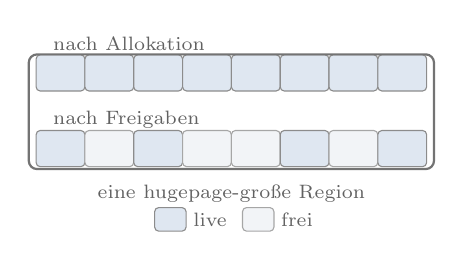
\begin{tikzpicture}[x=0.62cm,y=0.62cm]
      \node[faintlabel, anchor=west] at (-0.35,2.65) {nach Allokation};
      \foreach \i in {0,...,7} {
        \node[used] at (\i,2.05) {};
      }

      \node[faintlabel, anchor=west] at (-0.35,1.10) {nach Freigaben};
      \foreach \i/\style in {0/used,1/free,2/used,3/free,4/free,5/used,6/free,7/used} {
        \node[\style] at (\i,0.50) {};
      }

      \draw[draw=black!55,rounded corners=3pt,line width=0.8pt]
        (-0.65,0.08) rectangle (7.65,2.43);
      \node[faintlabel] at (3.5,-0.43) {eine hugepage-gro{\ss}e Region};

      \node[used, minimum width=0.40cm, minimum height=0.30cm] at (2.25,-0.95) {};
      \node[faintlabel, anchor=west] at (2.52,-0.95) {live};
      \node[free, minimum width=0.40cm, minimum height=0.30cm] at (4.05,-0.95) {};
      \node[faintlabel, anchor=west] at (4.32,-0.95) {frei};
    \end{tikzpicture}
  \end{column}
  \begin{column}{0.42\textwidth}
    \begin{itemize}
      \item Freier Speicher reicht nicht aus, wenn er zwischen live Objekten liegt
      \item Teilfreigabe kann RAM sparen, aber Hugepage-Abdeckung zerst\"oren
      \item Nichts freigeben kann TLB-Abdeckung halten, kostet aber Speicher
    \end{itemize}
    \vspace{0.5em}
    \begin{block}{Temeraire macht diesen Trade-off explizit.}
      Es packt kleine Objekte bewusst auf schon teilgef\"ullte Hugepages.
    \end{block}
  \end{column}
\end{columns}
\note{This figure comes from the report. The important point is not the drawing itself, but the conflict between RAM return and translation coverage.}
\end{frame}

\begin{frame}{Wo Temeraire in TCMalloc eingreift}
\begin{columns}[T,totalwidth=\textwidth]
  \begin{column}{0.52\textwidth}
    \centering
    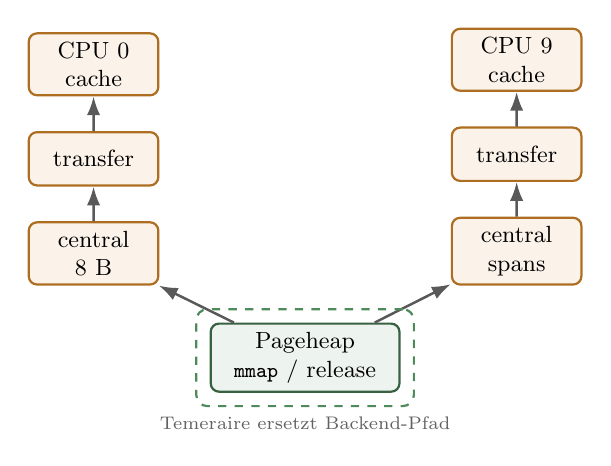
\begin{tikzpicture}[node distance=0.48cm and 0.58cm, scale=0.94, transform shape]
      \node[greenbox, minimum width=2.55cm] (os) {Pageheap\\\smallcode{mmap} / release};

      \node[orangebox, minimum width=1.75cm, above left=0.50cm and 0.68cm of os] (central8) {central\\8 B};
      \node[orangebox, minimum width=1.75cm, above right=0.50cm and 0.68cm of os] (centralbig) {central\\spans};

      \node[orangebox, minimum width=1.75cm, above=0.47cm of central8] (transfer8) {transfer};
      \node[orangebox, minimum width=1.75cm, above=0.47cm of centralbig] (transferbig) {transfer};

      \node[orangebox, minimum width=1.75cm, above=0.47cm of transfer8] (cpu0) {CPU 0\\cache};
      \node[orangebox, minimum width=1.75cm, above=0.47cm of transferbig] (cpu9) {CPU 9\\cache};

      \draw[arrow] (os) -- (central8);
      \draw[arrow] (os) -- (centralbig);
      \draw[arrow] (central8) -- (transfer8);
      \draw[arrow] (centralbig) -- (transferbig);
      \draw[arrow] (transfer8) -- (cpu0);
      \draw[arrow] (transferbig) -- (cpu9);

      \node[
        draw=temGreen,
        dashed,
        rounded corners=4pt,
        line width=0.8pt,
        fit=(os),
        inner sep=0.17cm,
        label={[faintlabel]below:Temeraire ersetzt Backend-Pfad}
      ] {};
    \end{tikzpicture}
  \end{column}
  \begin{column}{0.44\textwidth}
    \begin{itemize}
      \item Obere Caches bleiben TCMalloc
      \item Temeraire ersetzt den Backend-Pageheap
      \item Reproduktion vergleicht deshalb Legacy Pageheap gegen den
        hugepage-aware Pfad
    \end{itemize}
  \end{column}
\end{columns}
\end{frame}

\begin{frame}{Vier Komponenten teilen die Anfragen nach Gr\"o{\ss}e auf}
\centering
\resizebox{0.96\textwidth}{!}{%
\begin{tikzpicture}[
  >=Latex,
  font=\scriptsize,
  node distance=0.52cm and 0.62cm,
  every node/.style={align=center},
  allocatorbox/.style={
    draw=blue!60!black,
    fill=blue!12,
    rounded corners=4pt,
    line width=0.9pt,
    minimum width=3.0cm,
    minimum height=0.95cm,
    font=\small\ttfamily
  },
  cachebox/.style={
    draw=violet!70!black,
    fill=violet!15,
    rounded corners=4pt,
    line width=0.9pt,
    minimum width=2.55cm,
    minimum height=0.9cm,
    font=\small\ttfamily
  },
  fillerbox/.style={
    draw=green!50!black,
    fill=green!15,
    rounded corners=4pt,
    line width=0.9pt,
    minimum width=2.8cm,
    minimum height=0.9cm,
    font=\small\ttfamily
  },
  regionbox/.style={
    draw=orange!70!black,
    fill=orange!10,
    rounded corners=4pt,
    dashed,
    line width=0.9pt,
    minimum width=2.8cm,
    minimum height=0.9cm,
    font=\small\ttfamily
  },
  expl/.style={text width=8.55cm, align=left, font=\small},
  cue/.style={text width=11.95cm, align=left, font=\small}
]
\node[allocatorbox] (allocator) {HugeAllocator};
\node[expl, right=of allocator] {
  \faLayerGroup\quad holt ausgerichtete Hugepage-Bereiche vom System
};

\node[cachebox, below=of allocator] (cache) {HugeCache};
\node[expl, right=of cache] {
  \faArchive\quad h\"alt leere, bereits backed Hugepages zur Wiederverwendung
};

\node[fillerbox, below=of cache] (filler) {HugeFiller};
\node[expl, right=of filler] {
  \faCompress\quad packt kleine Allokationen auf teilbelegte Hugepages
};

\node[regionbox, below=of filler] (region) {HugeRegion};
\node[expl, right=of region] {
  \faExpand\quad behandelt mittlere Allokationen mit gr\"o{\ss}erem Rest
};

\node[cue, below=0.55cm of region, xshift=2.95cm] (redis) {
  \textbf{Routing:} $<1$ MiB $\rightarrow$
  \tikz[baseline=(tag.base)]{\node[fillerbox,minimum width=0pt,minimum height=0pt,
    inner sep=2.5pt,font=\scriptsize\ttfamily] (tag) {HugeFiller};};
  $1$ MiB--$1$ GiB $\rightarrow$
  \tikz[baseline=(tag.base)]{\node[cachebox,minimum width=0pt,minimum height=0pt,
    inner sep=2.5pt,font=\scriptsize\ttfamily] (tag) {HugeCache};}/
  \tikz[baseline=(tag.base)]{\node[regionbox,minimum width=0pt,minimum height=0pt,
    inner sep=2.5pt,font=\scriptsize\ttfamily] (tag) {HugeRegion};};
  $\geq1$ GiB $\rightarrow$
  \tikz[baseline=(tag.base)]{\node[cachebox,minimum width=0pt,minimum height=0pt,
    inner sep=2.5pt,font=\scriptsize\ttfamily] (tag) {HugeCache};}.
  Redis trifft vor allem den kleinen Pfad.
};
\end{tikzpicture}%
}
\note{This slide is the spoken legend for the previous figure. Keep it practical: allocator gets aligned hugepage ranges, cache reuses empty backed hugepages, filler handles the Redis-shaped small allocations, region catches medium allocations.}
\end{frame}

\begin{frame}{Redis-Hypothese}
\begin{columns}[T,totalwidth=\textwidth]
  \begin{column}{0.48\textwidth}
    \begin{block}{Workload aus dem Paper}
      \begin{itemize}
        \item Redis~6.0.9
        \item \smallcode{LPUSH} von f\"unf Werten
        \item \smallcode{LRANGE 0 4}
        \item 2000 Trials, je 1 Mio. Requests
      \end{itemize}
    \end{block}
  \end{column}
  \begin{column}{0.48\textwidth}
    \begin{block}{Erwarteter Effekt}
      Redis erzeugt viele kleine Listen- und String-Allokationen. Wenn
      \smallcode{HugeFiller} sie besser platziert, sinkt der TLB-Druck.
    \end{block}
    \vspace{0.4em}
    \[
      \text{kombiniert} =
      \frac{2}{1/r_{\mathrm{LPUSH}} + 1/r_{\mathrm{LRANGE}}}
    \]
  \end{column}
\end{columns}
\vspace{0.55em}
\begin{alertblock}{Konsequenz f\"ur die Messung}
Der erwartete Unterschied liegt unter einem Prozent. Reihenfolge, THP-Zustand
und Laufzeit-Validierung d\"urfen nicht implizit bleiben.
\end{alertblock}
\note{This is the handoff from mechanism to reproduction. The expected effect is small, so the rest of the talk is about removing easy sources of false signal.}
\end{frame}

\begin{frame}{Zwei Libraries machen den Vergleich m\"oglich}
\begin{columns}[T,totalwidth=\textwidth]
  \begin{column}{0.48\textwidth}
    \begin{block}{Rolle der Wrapper}
      Redis wird nicht zweimal umgebaut. Stattdessen werden zwei kleine
      TCMalloc-Shared-Libraries gebaut und beim Start in den Prozess geladen.
    \end{block}
    \vspace{0.45em}
    \begin{itemize}
      \item gleicher Redis-Build
      \item gleiche Wrapper-Quelle
      \item unterschiedliche TCMalloc-Backend-Konfiguration
    \end{itemize}
  \end{column}
  \begin{column}{0.48\textwidth}
    \begin{center}
    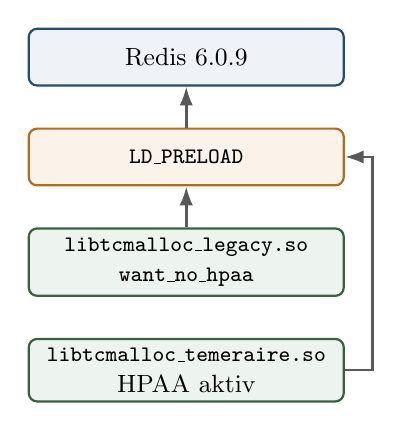
\begin{tikzpicture}[node distance=0.44cm]
      \node[box, minimum width=4.0cm] (redis) {Redis~6.0.9};
      \node[orangebox, minimum width=4.0cm, below=0.52cm of redis] (preload) {\smallcode{LD\_PRELOAD}};
      \node[greenbox, minimum width=4.0cm, below=0.52cm of preload] (legacy) {\smallcode{libtcmalloc\_legacy.so}\\\smallcode{want\_no\_hpaa}};
      \node[greenbox, minimum width=4.0cm, below=0.52cm of legacy] (tem) {\smallcode{libtcmalloc\_temeraire.so}\\HPAA aktiv};

      \draw[arrow] (preload) -- (redis);
      \draw[arrow] (legacy) -- (preload);
      \draw[arrow] (tem.east) -- ++(0.35,0) |- (preload.east);
    \end{tikzpicture}
    \end{center}
  \end{column}
\end{columns}
\vspace{0.25em}
\begin{alertblock}{Abgrenzung}
Der Wrapper ist kein neuer Allocator. Er macht den historischen TCMalloc-Code
preloadbar, damit der Legacy-vs.-Temeraire-Pfad messbar wird.
\end{alertblock}
\end{frame}

\begin{frame}{Der Wrapper musste in den historischen Build-Graph}
\begin{columns}[T,totalwidth=\textwidth]
  \begin{column}{0.48\textwidth}
    \begin{block}{Problem}
      Der Vergleich sollte nicht an selbst nachgebauten Link-Flags oder
      unvollst\"andigen TCMalloc-Abh\"angigkeiten h\"angen.
    \end{block}
    \vspace{0.45em}
    \begin{itemize}
      \item TCMalloc ist selbst ein Bazel-Projekt
      \item Abseil und interne Targets kommen aus dem nativen Build-Graph
      \item \smallcode{want\_no\_hpaa} ist ein TCMalloc-Target, kein Runtime-Flag
    \end{itemize}
  \end{column}
  \begin{column}{0.48\textwidth}
    \begin{center}
    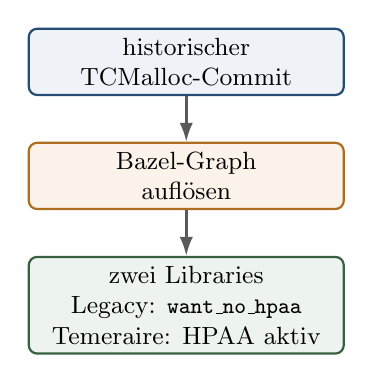
\begin{tikzpicture}[node distance=0.52cm]
      \node[box, minimum width=4.0cm] (src) {historischer\\TCMalloc-Commit};
      \node[orangebox, minimum width=4.0cm, below=0.58cm of src] (bazel) {Bazel-Graph\\aufl\"osen};
      \node[greenbox, minimum width=4.0cm, below=0.58cm of bazel] (out) {zwei Libraries\\Legacy: \smallcode{want\_no\_hpaa}\\Temeraire: HPAA aktiv};

      \draw[arrow] (src) -- (bazel);
      \draw[arrow] (bazel) -- (out);
    \end{tikzpicture}
    \end{center}
  \end{column}
\end{columns}
\vspace{0.1em}
\small
Bazel brachte TCMallocs Build-Graphen mit: Abseil, interne Targets und
Link-Semantik mussten nicht in CMake nachgebaut werden.
\end{frame}

\begin{frame}{Startpunkt: falsche N\"ahe zum Paper}
\begin{columns}[T,totalwidth=\textwidth]
  \begin{column}{0.49\textwidth}
    \begin{block}{Vorher}
      \begin{itemize}
        \item Redis~7.2.5 statt Redis~6.0.9
        \item glibc gegen gperftools
        \item kein Legacy-Pageheap gegen Temeraire
        \item Scope war anfangs zu breit formuliert
      \end{itemize}
    \end{block}
  \end{column}
  \begin{column}{0.47\textwidth}
    \begin{block}{Entscheidung}
      Das Artefakt wird auf den Redis-Case-Study-Teil eingegrenzt.
      Die Fleet- und Rollout-Ergebnisse bleiben au{\ss}erhalb der Reproduktion.
    \end{block}
    \vspace{0.45em}
    \begin{alertblock}{Erster Fix}
      Erst die Behauptung begrenzen, dann die Technik bauen.
    \end{alertblock}
  \end{column}
\end{columns}
\note{This slide starts the process narrative. It explains why the project was not just running an existing benchmark.}
\end{frame}

\begin{frame}{Umbau 1: Den richtigen Vergleich bauen}
\begin{center}
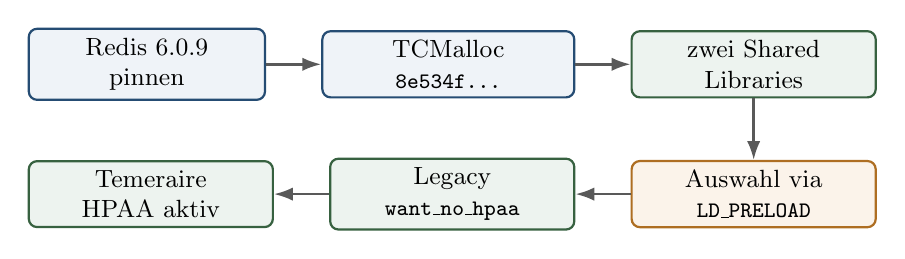
\begin{tikzpicture}[node distance=0.68cm]
  \node[box, minimum width=3.0cm] (redis) {Redis~6.0.9\\pinnen};
  \node[box, minimum width=3.2cm, right=0.7cm of redis] (tcmalloc) {TCMalloc\\\smallcode{8e534f...}};
  \node[greenbox, minimum width=3.1cm, right=0.7cm of tcmalloc] (libs) {zwei Shared\\Libraries};

  \node[orangebox, minimum width=3.1cm, below=0.78cm of libs] (preload) {Auswahl via\\\smallcode{LD\_PRELOAD}};
  \node[greenbox, minimum width=3.1cm, left=0.7cm of preload] (legacy) {Legacy\\\smallcode{want\_no\_hpaa}};
  \node[greenbox, minimum width=3.1cm, left=0.7cm of legacy] (tem) {Temeraire\\HPAA aktiv};

  \draw[arrow] (redis) -- (tcmalloc);
  \draw[arrow] (tcmalloc) -- (libs);
  \draw[arrow] (libs) -- (preload);
  \draw[arrow] (preload) -- (legacy);
  \draw[arrow] (legacy) -- (tem);
\end{tikzpicture}
\end{center}
\vspace{0.35em}
\begin{itemize}
  \item Der historische Commit enth\"alt noch den Schalter f\"ur den Legacy-Pfad
  \item Beide Varianten kommen aus derselben Wrapper-Quelle
  \item Die intendierte Differenz ist der TCMalloc-Backend-Pfad
\end{itemize}
\note{Stress the paired comparison. This is what makes the later result about Temeraire rather than about unrelated allocator implementations.}
\end{frame}

\begin{frame}{Fehlerbild: Build und Linkage}
\begin{columns}[T,totalwidth=\textwidth]
  \begin{column}{0.48\textwidth}
    \begin{block}{Was nicht sauber funktionierte}
      \begin{itemize}
        \item Moderner TCMalloc-Checkout passte nicht zur Wrapper-Strategie
        \item Externer Bazel-Wrapper erbte nicht alle Dependencies
        \item \smallcode{want\_no\_hpaa} war nicht global sichtbar
      \end{itemize}
    \end{block}
  \end{column}
  \begin{column}{0.48\textwidth}
    \begin{block}{Was am Ende funktionierte}
      \begin{itemize}
        \item Wrapper in \smallcode{tcmalloc/testing}
        \item Bazelisk und Bazel-Version pinnen
        \item LLVM-Pfad durch Make, Autotools und Bazel reichen
        \item fehlende Release-Symbole dynamisch aufl\"osen
      \end{itemize}
    \end{block}
  \end{column}
\end{columns}
\note{Keep this concrete. It shows why the final repo has wrapper logic and exact compiler plumbing instead of one clean build command.}
\end{frame}

\begin{frame}{Ein erfolgreicher Start beweist noch nicht den Allocator}
\begin{columns}[T,totalwidth=\textwidth]
  \begin{column}{0.52\textwidth}
    \begin{itemize}
      \item Redis kann weiter \smallcode{mem\_allocator: libc} melden
      \item Diese Meldung kommt aus der Redis-Build-Konfiguration
      \item F\"ur \smallcode{LD\_PRELOAD} z\"ahlt, was der Prozess wirklich mappt
    \end{itemize}
    \vspace{0.5em}
    \begin{block}{Pr\"ufung}
      \smallcode{/proc/\$pid/maps} muss die passende Library zeigen:
      \smallcode{libtcmalloc\_legacy.so} oder
      \smallcode{libtcmalloc\_temeraire.so}.
    \end{block}
  \end{column}
  \begin{column}{0.42\textwidth}
    \begin{center}
    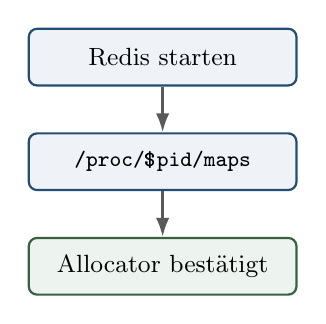
\begin{tikzpicture}[node distance=0.58cm]
      \node[box, minimum width=3.4cm] (launch) {Redis starten};
      \node[box, minimum width=3.4cm, below=0.58cm of launch] (maps) {\smallcode{/proc/\$pid/maps}};
      \node[greenbox, minimum width=3.4cm, below=0.58cm of maps] (ok) {Allocator best\"atigt};
      \draw[arrow] (launch) -- (maps);
      \draw[arrow] (maps) -- (ok);
    \end{tikzpicture}
    \end{center}
  \end{column}
\end{columns}
\note{This is a good place to mention that a benchmark can look successful while using the wrong allocator.}
\end{frame}

\begin{frame}{Ohne aktive Hugepages misst der Lauf nicht Temeraire}
\begin{columns}[T,totalwidth=\textwidth]
  \begin{column}{0.48\textwidth}
    \begin{alertblock}{Beobachtung in fr\"uhen Runs}
      \[
        \smallcode{AnonHugePages: 0\,kB}
      \]
      Redis lief, die Allocator-Varianten liefen, aber der Hugepage-Mechanismus
      war nicht belegt.
    \end{alertblock}
  \end{column}
  \begin{column}{0.48\textwidth}
    \begin{block}{Fix im Harness}
      \begin{itemize}
        \item \smallcode{thp-before.txt} und \smallcode{thp-after.txt}
        \item \smallcode{memory-sample-0250..2000.txt}
        \item \smallcode{smaps\_rollup} mit \smallcode{AnonHugePages}
        \item nur THP-aktive Runs f\"ur das Paper-Signal verwenden
      \end{itemize}
    \end{block}
  \end{column}
\end{columns}
\vspace{0.55em}
\begin{block}{Kriterium f\"ur g\"ultige Runs}
Sp\"atere Runs liefen mit \smallcode{[always] madvise never}; Redis-Snapshots
zeigten 14--18 MiB \smallcode{AnonHugePages} im Prozess. Erst dann war der
Hugepage-Pfad wirklich Teil der Messung.
\end{block}
\note{This is the main turning point. Earlier runs were useful engineering validation, but not evidence for the hugepage mechanism.}
\end{frame}

\begin{frame}{Der g\"ultige Lauf pr\"uft Aufbau, Mechanismus und Ergebnis}
\begin{center}
\resizebox{0.96\textwidth}{!}{%
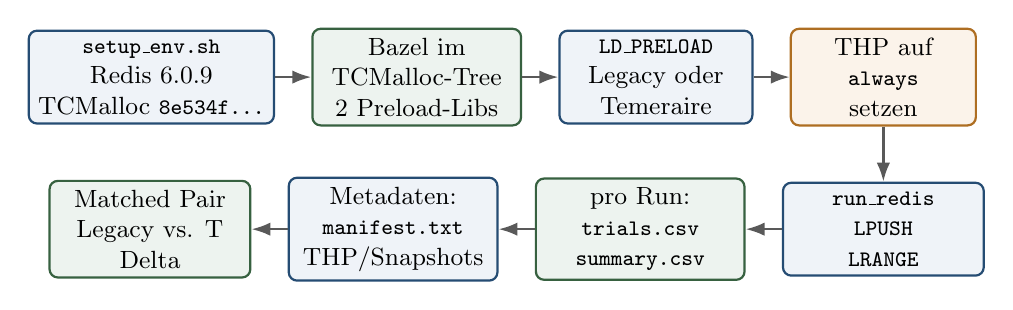
\begin{tikzpicture}[node distance=0.46cm and 0.46cm]
  \node[box, minimum width=2.55cm] (setup) {\smallcode{setup\_env.sh}\\Redis 6.0.9\\TCMalloc \smallcode{8e534f...}};
  \node[greenbox, minimum width=2.65cm, right=of setup] (libs) {Bazel im\\TCMalloc-Tree\\2 Preload-Libs};
  \node[box, minimum width=2.45cm, right=of libs] (preload) {\smallcode{LD\_PRELOAD}\\Legacy oder\\Temeraire};
  \node[orangebox, minimum width=2.35cm, right=of preload] (thp) {THP auf\\\smallcode{always}\\setzen};

  \node[box, minimum width=2.55cm, below=0.70cm of thp] (run) {\smallcode{run\_redis}\\\smallcode{LPUSH}\\\smallcode{LRANGE}};
  \node[greenbox, minimum width=2.65cm, left=of run] (snap) {pro Run:\\\smallcode{trials.csv}\\\smallcode{summary.csv}};
  \node[box, minimum width=2.65cm, left=of snap] (meta) {Metadaten:\\\smallcode{manifest.txt}\\THP/Snapshots};
  \node[greenbox, minimum width=2.55cm, left=of meta] (agg) {Matched Pair\\Legacy vs. T\\Delta};

  \draw[arrow] (setup) -- (libs);
  \draw[arrow] (libs) -- (preload);
  \draw[arrow] (preload) -- (thp);
  \draw[arrow] (thp) -- (run);
  \draw[arrow] (run) -- (snap);
  \draw[arrow] (snap) -- (meta);
  \draw[arrow] (meta) -- (agg);
\end{tikzpicture}%
}
\end{center}
\vspace{0.18em}
\begin{columns}[T,totalwidth=\textwidth]
  \begin{column}{0.48\textwidth}
    \begin{block}{\faCogs\quad Konfiguration}
      \footnotesize
      \begin{itemize}
        \item 2000 Trials; je 1 Mio. Requests
        \item 50 Clients, Pipeline 16
        \item ein Redis-Binary, zwei TCMalloc-\smallcode{.so}s
      \end{itemize}
    \end{block}
  \end{column}
  \begin{column}{0.48\textwidth}
    \begin{block}{\faClipboardCheck\quad Auswertung}
      \footnotesize
      \begin{itemize}
        \item LPUSH/LRANGE als harmonisches Mittel
        \item THP und \smallcode{AnonHugePages} protokolliert
        \item Delta nur im passenden Legacy/Temeraire-Paar
      \end{itemize}
    \end{block}
  \end{column}
\end{columns}
\note{This slide should be explained as the actual handoff chain: setup creates two preload libraries, the runner selects one library per Redis process, and the aggregator only compares matched legacy/Temeraire summaries.}
\end{frame}

\begin{frame}{Release-on war faktisch nicht eingeschaltet}
\begin{columns}[T,totalwidth=\textwidth]
  \begin{column}{0.48\textwidth}
    \begin{block}{\faPlayCircle\quad Was lief}
      \begin{itemize}
        \item Background-Thread gestartet
        \item Per-CPU-Caches wurden gepflegt
      \end{itemize}
    \end{block}
  \end{column}
  \begin{column}{0.48\textwidth}
    \begin{alertblock}{\faExclamationTriangle\quad Was fehlte}
      Release-Rate nicht gesetzt: TCMalloc blieb bei \smallcode{0 B/s}.
      Damit gab es keine periodische Pageheap-Freigabe.
    \end{alertblock}
  \end{column}
\end{columns}
\vspace{0.5em}
\begin{block}{Konsequenz}
  Die alten Werte waren kein Release-on-Ergebnis. Der korrigierte Lauf setzt
  eine positive Rate explizit; das Paper nennt seine Rate nicht.
\end{block}
\note{This is a correction to the experimental record, not a minor caveat. The release-on logs remain useful for diagnosing the setup, but they cannot support a claim about periodic pageheap release.}
\end{frame}

\begin{frame}{Release-off liegt nahe am kleinen Paper-Effekt}
\begin{columns}[T,totalwidth=\textwidth]
  \begin{column}{0.50\textwidth}
    \centering
    \small
    \begin{tabular}{@{}lcc@{}}
      \toprule
      Run & Reihenfolge & Delta \\
      \midrule
      THP fixed-order & L first & \pct{+1.88} \\
      balanced 1 & L first & \pct{+0.43} \\
      balanced 2 & T first & \pct{+0.48} \\
      balanced 3 & L first & \pct{-0.76} \\
      balanced 4 & T first & \pct{+3.46} \\
      \bottomrule
    \end{tabular}
  \end{column}
  \begin{column}{0.46\textwidth}
    \begin{block}{Befund}
      Vier von f\"unf THP-aktiven vollst\"andigen Runs favorisieren Temeraire.
      Der Median liegt bei \pct{+0.48}.
    \end{block}
    \vspace{0.45em}
    \begin{block}{Paper-Vergleich}
      Redis$^\dagger$ im Paper: \pct{+0.75}\\
      Periodic release disabled.
    \end{block}
  \end{column}
\end{columns}
\note{This is the strongest result. It is still small and noisy, but it is repeatedly in the paper's direction.}
\end{frame}

\begin{frame}{Die alten Release-on-Runs bleiben nur als Fehlerprotokoll}
\begin{columns}[T,totalwidth=\textwidth]
  \begin{column}{0.47\textwidth}
    \centering
    \color{temOrange}\fontsize{31}{34}\selectfont\faBug
    \par\vspace{0.35em}
    \color{temDark}\Large\smallcode{release-on}\par
    \vspace{0.15em}
    \normalsize effektiv \smallcode{0 B/s}
  \end{column}
  \begin{column}{0.49\textwidth}
    \begin{alertblock}{Kein Paper-Vergleich}
      Der Manifestname versprach eine Bedingung, die der Prozess nicht erf\"ullte.
    \end{alertblock}
    \vspace{0.4em}
    \begin{block}{Warum die Logs bleiben}
      Sie dokumentieren den Konfigurationsfehler und die lokale Streuung. Die
      Deltas werden nicht als Ergebnis verwendet.
    \end{block}
  \end{column}
\end{columns}
\note{Keep the numbers visible as part of the experimental record. Their status has changed: they document the misconfigured condition, not the paper's release-on case.}
\end{frame}

\begin{frame}{Drei Release-Raten ergeben keinen stabilen Trend}
\centering
\small
\begin{tabular}{@{}lrrrrr@{}}
  \toprule
  Rate & Pair 1 & Pair 2 & Pair 3 & Pair 4 & Median \\
  \midrule
  16 MiB/s  & \pct{+1.91} & \pct{-0.16} & \pct{-0.27} & \pct{-1.37} & \pct{-0.21} \\
  64 MiB/s  & \pct{-6.88} & \pct{+2.10} & \pct{+11.49} & \pct{+12.21} & \pct{+6.80} \\
  256 MiB/s & \pct{+15.73} & \pct{-0.09} & \pct{+0.50} & \pct{-0.77} & \pct{+0.20} \\
  \bottomrule
\end{tabular}
\vspace{0.55em}
\begin{columns}[T,totalwidth=\textwidth]
  \begin{column}{0.48\textwidth}
    \begin{block}{Was jetzt stimmt}
      24 Allocator-Runs, je 2000 Trials. Jeder Redis-Log best\"atigt die
      positive Release-Rate.
    \end{block}
  \end{column}
  \begin{column}{0.48\textwidth}
    \begin{alertblock}{Was das Ergebnis begrenzt}
      Kein monotoner Rate-Effekt. Absolute Leistung fiel zeitweise um mehr als
      20\% und erholte sich sp\"ater wieder.
    \end{alertblock}
  \end{column}
\end{columns}
\note{The corrected mechanism works, but the host is not stable enough for a clean sub-one-percent comparison. The 64 MiB/s median and the first 256 MiB/s pair are driven by large throughput shifts between consecutive hour-long runs.}
\end{frame}

\begin{frame}{Host-Drift ist gr\"o{\ss}er als der erwartete Effekt}
\begin{columns}[T,totalwidth=\textwidth]
  \begin{column}{0.49\textwidth}
    \begin{block}{Auswertbarer Befund}
      Release-off liegt mit \pct{+0.48} Median im kleinen Effektbereich des
      Paper-Werts von \pct{+0.75}. Die f\"unf Run-Paare streuen jedoch deutlich.
    \end{block}
  \end{column}
  \begin{column}{0.47\textwidth}
    \begin{block}{Korrigierter Befund}
      Release-on ist technisch korrekt gemessen, zeigt aber keinen stabilen
      Rate-Trend. Host-Drift ist gr\"o{\ss}er als der Paper-Effekt.
    \end{block}
  \end{column}
\end{columns}
\vspace{0.55em}
\begin{alertblock}{Vertretbare Aussage}
Das Artefakt rekonstruiert den Redis-Vergleich mit \"offentlichem Code.
Der korrigierte Lauf zeigt vor allem die Grenze konsekutiver Ein-Stunden-Runs.
\end{alertblock}
\note{This is the thesis of the final result. Keep the wording cautious and concrete.}
\end{frame}

\begin{frame}{Was diese Reproduktion nicht zeigen kann}
\begin{columns}[T,totalwidth=\textwidth]
  \begin{column}{0.48\textwidth}
    \begin{block}{Nicht reproduziert}
      \begin{itemize}
        \item Google-Fleet-Experiment
        \item Produktions-Rollout
        \item interne Allocator-Binaries
        \item exakte Paper-Hardware
      \end{itemize}
    \end{block}
  \end{column}
  \begin{column}{0.48\textwidth}
    \begin{block}{Lokale Abweichungen}
      \begin{itemize}
        \item Docker/WSL2 und geteilter Kernel
        \item Consumer i7 statt Skylake Xeon Server
        \item THP-Policy aus der Host/VM-Umgebung
        \item Public TCMalloc als historische Ann\"aherung
      \end{itemize}
    \end{block}
  \end{column}
\end{columns}
\vspace{0.5em}
\begin{block}{Nutzen der Grenzen}
Sie trennen den methodisch reproduzierten Redis-Pfad von den Teilen des Papers,
die ohne Google-Infrastruktur nicht nachstellbar sind.
\end{block}
\note{Limitations define what the artifact can claim.}
\end{frame}

\begin{frame}{Fazit}
\begin{columns}[T,totalwidth=\textwidth]
  \begin{column}{0.53\textwidth}
    \begin{block}{Technische Lektion}
      Der schwere Teil war nicht \smallcode{redis-benchmark}, sondern der Weg zu
      einem echten Legacy-vs.-Temeraire-Vergleich mit aktiven Hugepages.
    \end{block}
    \vspace{0.5em}
    \begin{itemize}
      \item Vergleich aus public TCMalloc rekonstruiert
      \item Preload zur Laufzeit validiert
      \item THP-Fehlerbild gefunden und instrumentiert
      \item Release-on korrigiert und mit drei Raten neu gemessen
    \end{itemize}
  \end{column}
  \begin{column}{0.43\textwidth}
    \begin{alertblock}{Endstand}
      Release-off zeigt ein kleines positives Mediansignal bei hoher Streuung.
      Release-on ist aktiv, aber Host-Drift verhindert ein stabiles Ergebnis.
    \end{alertblock}
  \end{column}
\end{columns}
\note{Close by returning to the narrative: mechanism, broken assumptions, corrected experiment, cautious result.}
\end{frame}

\end{document}
